\section{Web Information Systems}

\subsection{Introduction and Definition of WIS}\label{introduction-to-web-information-systems}

Good morning! In this class, we will be discussing web information
systems. As usual, you can find the slides on WEBEEP. Let's begin by
defining what a web information system is.

\begin{figure}[!h]
  \centering
  \includegraphics[page=2, trim = 2cm 3cm 2cm 4.5cm, clip, width=\textwidth]{images/03 - Web_Information_Systems.pdf}
\end{figure}

A web information system is a system that facilitates communication
between machines using either the public internet or an IP-based private
VPN. Users can access the system's functionalities through a web
browser. This definition provides a broad understanding of what a web
information system entails.

\paragraph*{Defining Web Information Systems}
The public internet and the IP protocol, along with browsers, have
brought about significant changes in information systems. Any system
that meets two criteria can be considered a web information system.
Firstly, it must be accessible through a browser. Secondly, it should be
connected to the private VPN of the company. This means that even a
traditional ERP with its core functionalities can be classified as a web
information system if it meets these criteria.


\subsection{Impact of Technical Innovations}
These two technical
innovations---internet and browsers (user interfaces)---have resulted in a transformation of the technologies
utilized, even by components of web information systems that were
created prior to the advent of the web. In essence, ERP providers have
reimagined the interface and core technologies of their packages to
align with this new paradigm.

\subsubsection{The Internet and Its
  Influence}\label{the-internet-and-its-influence}

\begin{figure}[!h]
  \centering
  \includegraphics[page=4, trim = 2cm 2.5cm 2cm 1cm, clip, width=\textwidth]{images/03 - Web_Information_Systems.pdf}
\end{figure}

Now, let's discuss the main innovation that revolutionized web
information systems: the internet. The internet connected companies to
individual customers for the first time, marking a significant change in
the business landscape. This not only impacted individual customers but
also the employees working for these companies. The ability to connect
the company's potential market, especially retail customers, through a
public network was seen as a monumental shift.

During the late 90s, when the internet was introduced, there was a great
deal of hope and belief in the transformative power of this new
technology. There was a hype surrounding the web, with expectations that
it would drastically change people's lives in a short period of time.
The paradigm of exponential organization emerged, where companies
without the burden of physical shops or channels to reach customers
could experience rapid growth. As a result, the value of web-based
companies experienced significant growth around the year 2000.

\paragraph{The Dot Com Bubble}\label{the-dot-com-bubble}

The dot com bubble refers to a period when the value of stocks of
companies with websites ending in ``.com'' skyrocketed, far exceeding
their actual revenues and assets. However, this rapid growth was
eventually followed by a significant stock market crash, one of the
largest in recent history. This sudden shift from extreme optimism to
pessimism marked a turning point in the market.

\paragraph{Web Technology in Traditional
  Companies}\label{web-technology-in-traditional-companies}

The web has undoubtedly revolutionized processes for both traditional
and new companies, creating new industries while also causing the
decline of others. However, the pace at which society adapted to these
changes was slower than the expectations of the stock exchange. For
traditional companies to fully benefit from web innovation, they must
first go through the implementation and integration of their information
systems, even with traditional technologies. Without this, it is
challenging for them to compete effectively on the web, unless they have
a history of being highly innovative in their approach to information
systems and are prepared to utilize the web as a new channel to reach
customers.

For instance, companies that lack a unified data system, which is a
fundamental aspect of the ERP paradigm, will struggle to provide a
satisfactory web service. The web is a more objective platform compared
to a physical store, as there is no personal interaction. Customers have
certain expectations for service quality, which are set by industry
leaders. Consequently, the web can actually make the customer
relationship more challenging rather than easier. Only companies that
have successfully integrated previous technologies into their operations
have been able to fully exploit the potential of the web.

\paragraph{Extended ERP and E-Commerce}\label{extended-erp-and-e-commerce}

When examining the functional architecture of ERP systems, it becomes
clear that extended ERP is more influenced by the web than core ERP. The
web has opened up new opportunities, particularly in e-commerce, which
continues to evolve. Extended ERP, which is enabled by the web,
encompasses various functionalities that must be supported by a
well-integrated and IT-supported internal process.

One of the key enabling technologies for extended ERP is CRM, with the
web playing a significant role. While companies have been using
technology, such as Salesforce automation, to interact with customers
for some time, the web has made it easier to showcase services, prices,
and conditions, as well as compare alternative suppliers. This has
created a need for integration across different channels, as any
mistakes or inaccuracies on the web are visible to all. It is no longer
acceptable for customers to have to visit a retail shop for information;
it must be readily available and accurate on the web.

\section{E-Commerce and Its
  Evolution}\label{e-commerce-and-its-evolution}

Companies have recognized the importance of integrating customer
information into a single database, commonly known as a customer
database or CRM. This integration, whether referred to as omni-channel
or multi-channel, has become increasingly important as the web has
become the primary access point for both customers and internal users.

\begin{figure}[!h]
  \centering
  \includegraphics[page=5, trim = 2cm 5cm 2cm 4.5cm, clip, width=\textwidth]{images/03 - Web_Information_Systems.pdf}
\end{figure}

Initially, the web was seen as a platform for e-commerce, allowing
companies to sell their products online and reach a wider market. This
was seen as a significant opportunity. E-commerce refers to the buying
and selling of products and services online, primarily targeting retail
customers. On the other hand, when referring to business customers, the
term e-business is used. For example, if a company purchases from
another company online, it is considered e-business. Similarly, if a
public administration buys from a supplier online or provides services
to other public institutions or citizens, it is referred to as
e-government.

In summary, e-commerce focuses on reaching the market and selling
products online, while e-business and e-government encompass a broader
range of online transactions involving business customers and public
administrations, respectively.

\section{The Dot Com Trend and Its
  Aftermath}\label{the-dot-com-trend-and-its-aftermath}

In the early days of the dot com trend, many companies initially set up
their e-commerce operations as separate units or even separate
companies. This was a common approach when a new technology brought
about significant changes. These companies lacked the necessary
expertise to effectively manage and leverage the new technology, so they
sought the help of consultants and formed internal teams to handle it.
Over time, these teams evolved into dedicated units focused on the new
technology, such as the web.

\begin{figure}[!h]
  \centering
  \includegraphics[page=6, trim = 1.5cm 4cm 2cm 3cm, clip, width=\textwidth]{images/03 - Web_Information_Systems.pdf}
\end{figure}

This pattern of innovation is not unique to the web; it has been
observed in various industries. However, during the dot com era,
companies that were perceived as pure dot coms, operating solely on the
web without any traditional brick-and-mortar presence, were highly
valued in the stock market. This led even traditional companies to
establish separate units or even separate companies with their own
distinct brands to tap into the potential of the web. For instance, in
2000, Deutsche Bank launched Bank 24, a web-only bank operating as a dot
com.

However, this trend came to a halt after the dot com bubble burst and
the subsequent stock market failure. Even Deutsche Bank eventually
integrated Bank 24 back into its core services, recognizing the need to
reassess their approach in light of the challenges faced by dot com
companies.

\section{Integrating Web and Traditional
  Channels}\label{integrating-web-and-traditional-channels}

Companies have recognized the importance of integrating the web as an
additional channel for their existing customers. There are a few reasons
behind this realization. Firstly, companies understood that relying
solely on the web for growth and stock market success was no longer
feasible after the dot com bubble burst. Secondly, they realized that
web-based operations still require physical processes and the management
of people, offices, and complementary services. This led to the
recognition of the synergies between web-based companies and traditional
structures, as Deutsche Bank recognized.

To leverage these synergies, companies brought web-based operations back
into their traditional structures and began integrating the web as a
channel alongside other existing channels. This integration process was
facilitated by customer relationship management (CRM) practices.
Companies started by creating a shared customer database and analyzing
it to understand the evolving habits of web customers. Based on these
insights, they developed innovative services to cater to the changing
needs of web customers over time.

\begin{figure}[!h]
  \centering
  \includegraphics[page=7, trim = 2cm 1.5cm 2cm 1.5cm, clip, width=\textwidth]{images/03 - Web_Information_Systems.pdf}
\end{figure}

Initially, customers were skeptical about making purchases on the web,
especially for high-value or high-quality products. They preferred
traditional brick-and-mortar shops. However, over time, customer
behavior shifted, and e-commerce gained traction across various
industries. The pace of this shift varied across industries, with some
experiencing faster adoption than others. Nevertheless, e-commerce has
become prevalent in almost all industries, including fashion, grocery,
tourism, banking, trading, and learning. Each industry has its own
specific terms and practices related to e-commerce.

\section{The Role of E-Commerce
  Post-COVID-19}\label{the-role-of-e-commerce-post-covid-19}

When the internet was first introduced, there were predictions about
which industries would be most impacted by e-commerce and how quickly it
would replace traditional channels. However, it took nearly 20 years for
e-commerce to become pervasive, serving only a small percentage of
transactions and clients. The COVID-19 pandemic changed this
dramatically, giving e-commerce a significant boost. It quickly
developed and penetrated the market, reaching a larger audience. While
there has been a slight decline after the initial surge, e-commerce has
still experienced substantial growth and increased penetration.

\section{Customer Journey and Online
  Information}\label{customer-journey-and-online-information}

To illustrate this point, let's consider the example of grocery
shopping. Despite the pandemic, only a small percentage of people
actually do their grocery shopping online. This indicates that the
experience of shopping in a traditional store or through traditional
distribution methods is still considered superior to the online
experience. As a result, the current trend is to view online shopping as
complementary to other channels, rather than a standalone option.

\begin{figure}[!h]
  \centering
  \includegraphics[page=8, trim = 1.5cm 3cm 2cm 3cm, clip, width=\textwidth]{images/03 - Web_Information_Systems.pdf}
\end{figure}

When customers engage with a company, they go through a journey that
involves multiple channels at different stages of the transaction. It
all begins with a need, which may arise from seeing an advertisement or
simply having a requirement. The first step in this journey is typically
going online to gather information. This initial step is crucial in the
transaction process and is usually done through the web. When customers
are unsure of where to make a purchase, they turn to the internet to
find information. This helps them make decisions about the provider, the
brand, and the specific product they want to buy. With the advent of
social media, customers also rely on product reviews to guide their
choices. This search phase of the transaction, where customers seek
information, accounts for approximately 90\% of visits to a company's
website.

\section{Designing Effective Web
  Information}\label{designing-effective-web-information}

The main purpose of websites is to provide information to customers who
are looking for products or learning about a company for the first time.
Typically, websites include a general presentation of the company, its
mission, organizational structure, job opportunities, news and events,
and information about its products. Some older websites may offer a
downloadable product catalog in PDF format or a multimedia online
catalog where customers can browse through the products. These websites
often provide recommendations for related products that are commonly
purchased together. Contact information, such as the call center,
company size, and location, is also provided, sometimes with a map for
easy navigation.

When designing the information services of their website, companies are
primarily concerned with providing a positive first impression to
customers who have no prior knowledge of the company. This can be
challenging for companies, as they need to carefully design the
website's navigation structure. It is often best to follow a navigation
structure that is similar to what competitors use, as customers have
certain expectations about where to find specific information on a
company's homepage. Keeping the information provided on the website
standardized is a good idea, although it should be regularly updated as
company information, including the mission, can change over time. To
update the information on their website, companies need to gather the
necessary information from various stakeholders within the organization
who possess the relevant knowledge. This can be a complex task, as
information is often scattered across different departments or
individuals. The website serves as a central access point for customers
to find all the information they need.

\section{Quality Criteria for E-Commerce
  Sites}\label{quality-criteria-for-e-commerce-sites}


\begin{figure}[!h]
  \centering
  \includegraphics[page=9, trim = 1.5cm 4.5cm 3cm 4cm, clip, width=\textwidth]{images/03 - Web_Information_Systems.pdf}
\end{figure}

In order to provide consistent information to customers on the web,
information owners must cooperate. There are two approaches to
collecting this information. The first approach is federated, where
there is one central site with a thin layer of information and multiple
local sites where individual business units can provide their own
information. The landing page serves as a collection of links to the
different business units' websites. While this approach allows for
information retrieval to be closer to the business units, it often
results in a website that lacks standardization and has lower overall
quality.

The second approach is to establish an editorial committee that
constantly updates the information on the website. This committee seeks
information from the different business units and follows a common
template for all units, ensuring standardization. Although this approach
is more expensive due to the need for an editorial committee and
agreement on the information to be provided, it generally leads to
higher quality.

\begin{figure}[!h]
  \centering
  \includegraphics[page=10, trim = 2cm 2cm 2cm 4cm, clip, width=\textwidth]{images/03 - Web_Information_Systems.pdf}
\end{figure}

When considering the quality criteria for an e-commerce site, there are
several factors to consider. First, customers expect the content to be
complete, dependable, and correct. They also want consistency in the
information provided by the call center. Second, the structure of the
website should allow customers to easily navigate and understand the
information. A centralized structure is preferable in this regard. The
presentation of the website should have a coherent graphic style to
instill trust and confidence in the company. The layout and position of
information should be intuitive and standardized. Navigation should also
be intuitive, with multiple paths to reach the same information. The
website should be well-connected, allowing customers to navigate between
pages without having to return to the homepage. The ease of navigation,
including the ability to go back multiple steps, is crucial.

In conclusion, the quality criteria for an e-commerce site include
content completeness and dependability, a clear and intuitive structure,
a coherent graphic style, and easy navigation with multiple paths to
reach information.